%% Preamble
% Document type, packages imported, theme and color:
\documentclass{beamer}
\usepackage{amsmath,geometry,graphicx}
\usetheme{Madrid}
\usepackage{multicol}

% Title page
\title{Light reflections}

\date{July 25, 2018}
\author{
Michael Byrne, 
Fatoumata Sanogo,
Pai Song,
Kevin Tsai,
Hang Yang, and
Li Zhu\\
\medskip
Problem Presenter:  John Peach (MIT Lincoln Lab)\\
Faculty Mentor: Alen Alexanderian (NCSU)
}
\titlegraphic{}
\institute[Abbreviation]{SAMSI-IMSM}

%% Presentation
\begin{document}

\begin{frame}[t] 
\frametitle{Motivation} 
\begin{itemize} 
\item Satellite tracking 
\item Prediction of reflective response 
\end{itemize} 
\centerline{\includegraphics[width = 0.75\linewidth]{./figs/Satellite.jpg}} 
\end{frame} 
 
\begin{frame}[t] 
\frametitle{Goals} 
\begin{itemize} 
\item Build complex objects using various methods (OpenSCAD, R-functions) 
\item Develop a continuous approach to optical cross section (OCS) computation 
\item Find a solution to the mutlipath problem 
\end{itemize} 
\centerline{\includegraphics[width = 0.9\linewidth]{rocket.pdf}} 
\end{frame} 


\begin{frame}
\frametitle{OpenSCAD} 
\centerline{\includegraphics[scale = 0.3]{./figs/sdh_mesh}} 
\end{frame}

\begin{frame}[t] 
\frametitle{R-functions} 
\begin{itemize} 
\item Known also as Rvachev functions (1963) 
\item Uses Boolean algebra to construct composite shapes from simple shapes 
\item Implicit surface representation 
\end{itemize} 
${\left(x-\frac{3}{2}\right)}^2-\sqrt{{\left(x^2+y^2+z^2-1\right)}^2+{\left({\left(x-\frac{3}{2}\right)}^2+y^2+z^2-1\right)}^2}+x^2+2\,y^2+2\,z^2-2 = 0$ 
\centerline{\includegraphics[width = 0.75\linewidth]{./figs/TwoSpheres}} 
\end{frame} 

\begin{frame}
\frametitle{R-function examples} 
\centerline{\includegraphics[width=.32\textwidth]{./figs/shape1.pdf} \: \includegraphics[width=.32\textwidth]{./figs/shape2.pdf}}  
\includegraphics[width=.32\textwidth]{./figs/union.pdf} 
\includegraphics[width=.32\textwidth]{./figs/intersect.pdf} 
\includegraphics[width=.32\textwidth]{./figs/diff.pdf} 
\end{frame} 
\end{frame}

\begin{frame}[t]
\frametitle{Optical cross section}
\begin{itemize}
\item Accumulated reflectance over a target surface
\item Discrete: summing triangular facets (5 -- 20,000+) 
\item Continuous: chebfun in conjunction with R-functions
\end{itemize}
\centerline{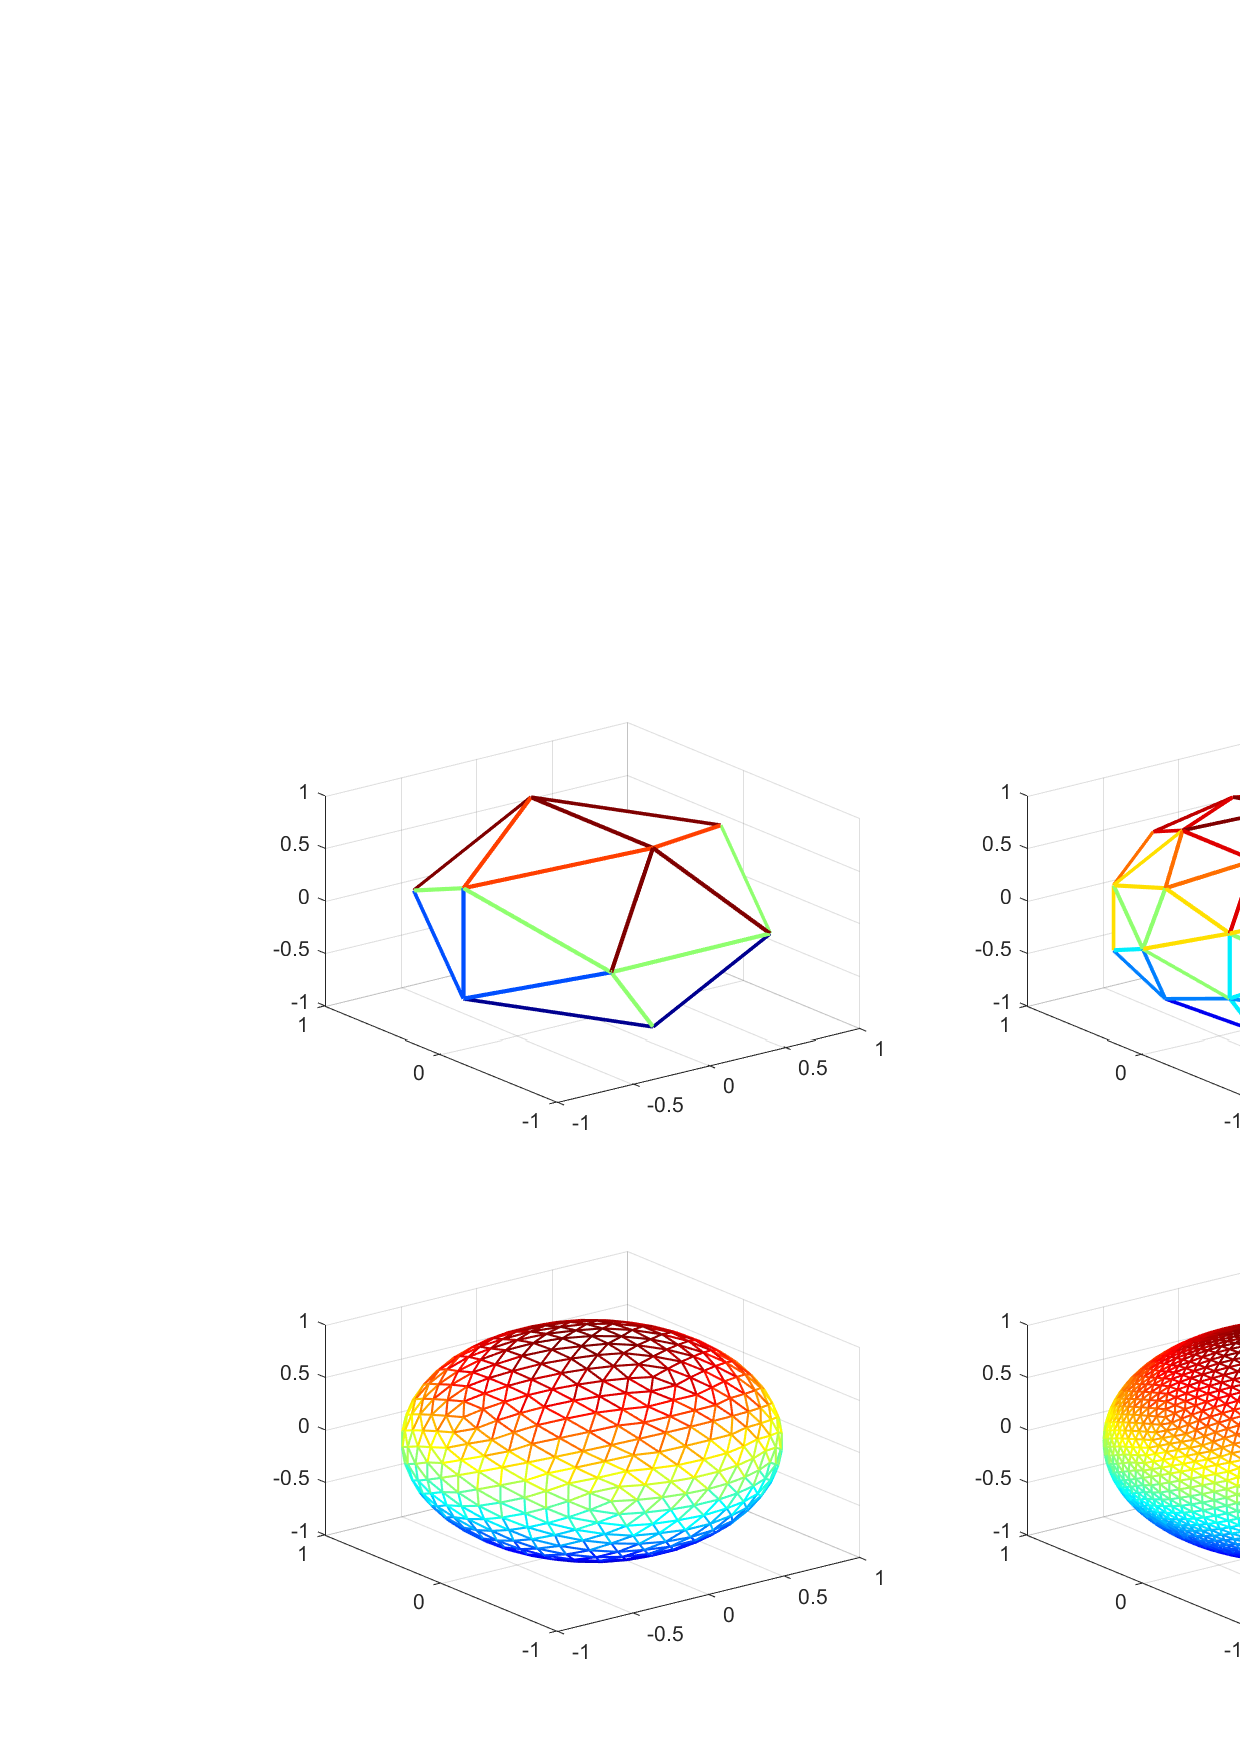
\includegraphics[scale = 0.5]{./figs/facet.png} \: 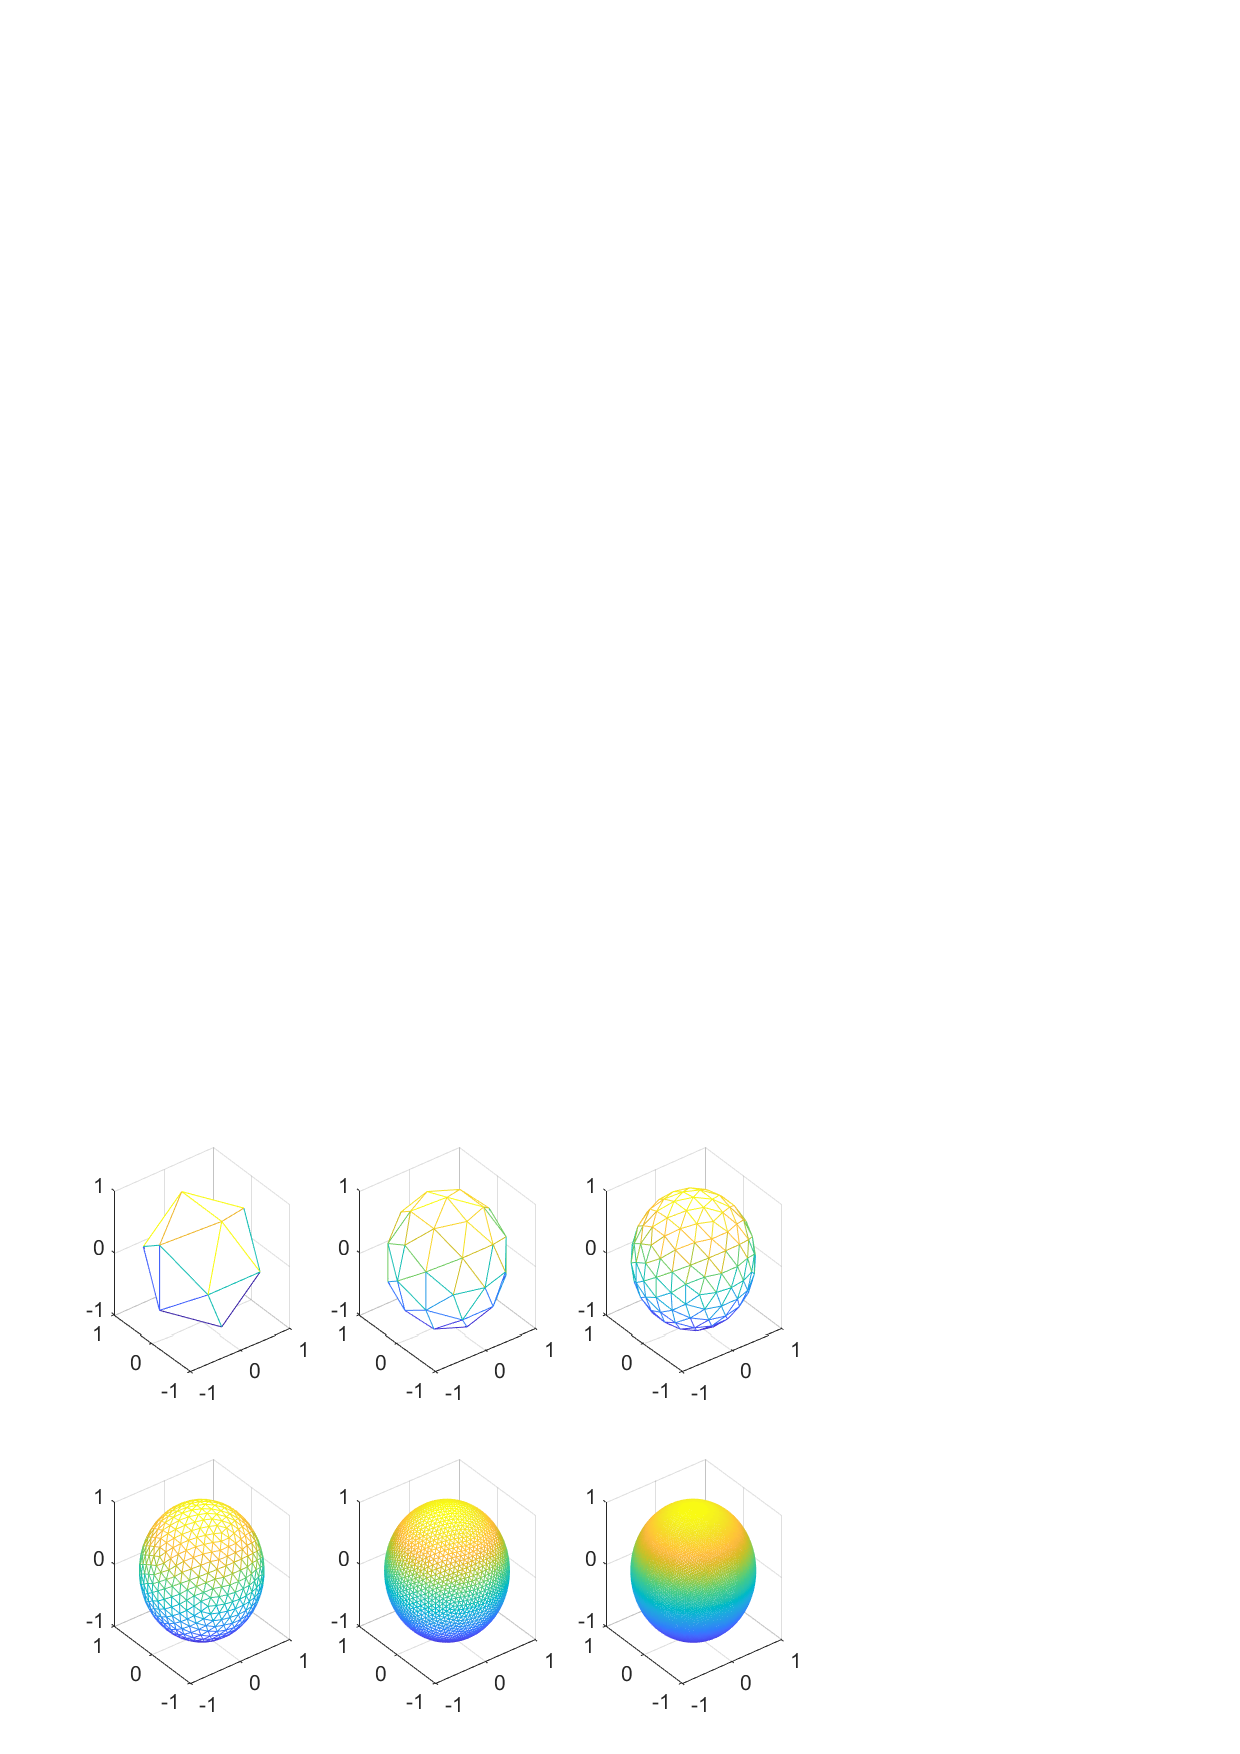
\includegraphics[scale = 0.5]{./figs/icosahedron.png}}
\end{frame}

\begin{frame}[t]
\frametitle{Chebfun and the sphere}
\begin{itemize}
\item Unit sphere (spherical coordinate)
\item Light source: fixed at the direction $(\theta,\phi) = (\frac{\pi}{2},\frac{\pi}{2})$
\item Detector: orbiting on $xy$-plane
\item Varying specular highlight
\end{itemize}
\begin{multicols}{2}
\centering \includegraphics[scale=0.13]{./figs/OCS_parallel_plane}
\begin{figure}
\centering \includegraphics[scale=0.1]{./figs/orbiting_example}\caption{qimono.
 pixabay. 2016}
\end{figure}
\end{multicols}
\end{frame}

\begin{frame}[t]
\frametitle{Chebfun and the sphere (cont'd)}
\begin{itemize}
\item Unit sphere
\item Light source: fixed at the direction $(\theta,\phi) = (0,0)$
\item Detector: orbiting on $xy$-plane
\item Varying specular highlight
\end{itemize}

\centering \includegraphics[scale=0.13]{./figs/OCS_perpendicular_plane}
\end{frame}


\begin{frame}[t]
\frametitle{Multipath}
\end{frame}


\begin{frame}[t]
\frametitle{Conclusion and future work}
\begin{itemize}
\item Implicit representations of composite objects readily obtained from R-functions 
\item Advantages of continuous OCS computation over facet method for simple shapes
\item 
\item Investigation of continuous solutions for more complex/``sharper" objects 
\end{itemize}
\end{frame}

\end{document}


%% Image references: 
 
% Satellite.jpg: https://www.newscientist.com/article/2113311-first-ever-lightning-mapping-satellite-set-for-take-off/ 
 